\section{System Architecture \& Control Plane}
\label{sec:architecture}

DRIGS is designed around a decoupled, layered micro-architecture that strictly isolates domain scheduling policies from lower-level execution primitives and vendor hardware APIs. This architectural separation allows DRIGS to operate natively across diverse deployment targets—from local multi-GPU workstations to dynamic, ephemeral cloud notebook instances (e.g., Kaggle, Google Colab)—without requiring root access or container privileges.

\subsection{Architectural Overview}
\begin{figure*}[t]
    \centering
    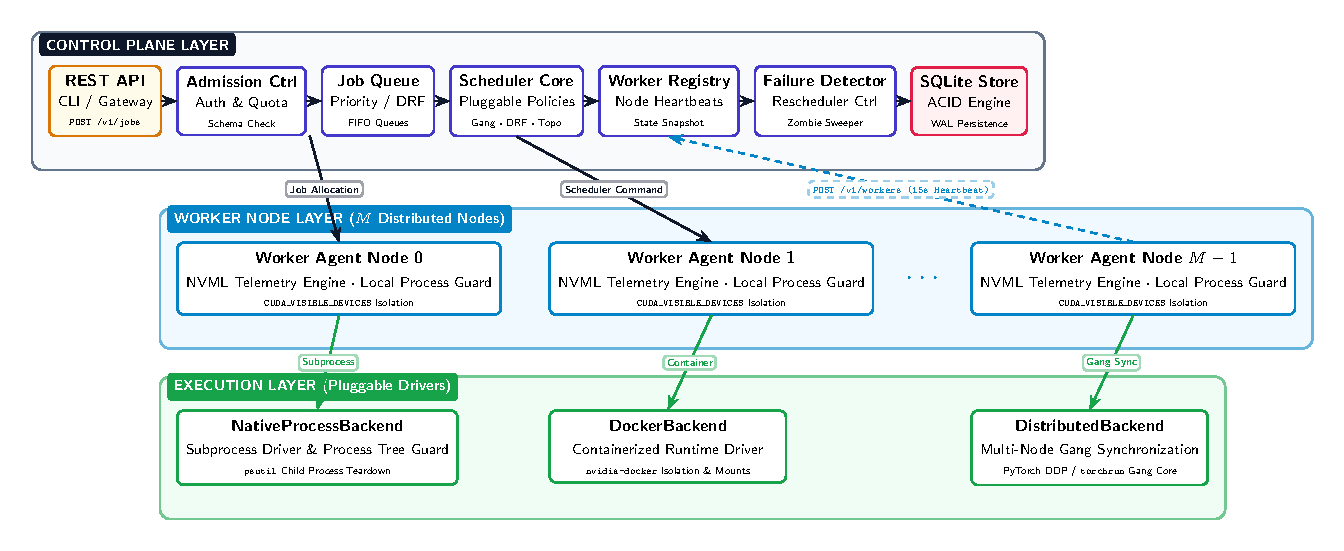
\includegraphics[width=\linewidth]{figures/architecture.pdf}
    \caption{DRIGS three-layer system architecture. The Control Plane orchestrates job admission, priority queueing, pluggable scheduling, and worker lifecycle management. Worker Node Agents perform real-time NVML hardware telemetry and report heartbeats. The Execution Layer provides modular process backends (native, Docker, distributed).}
    \label{fig:architecture_overview}
\end{figure*}

Figure~\ref{fig:architecture_overview} illustrates the high-level architecture of DRIGS. The system is organized into three distinct layers:
\begin{enumerate}
    \item \textbf{Control Plane Layer:} Manages job submission validation (\texttt{AdmissionController}), priority job queueing (\texttt{JobQueue}), pluggable scheduler evaluation (\texttt{Scheduler}), worker lifecycle registry (\texttt{WorkerRegistry}), and failure detection/recovery (\texttt{FailureDetector}, \texttt{Rescheduler}).
    \item \textbf{Worker Node Layer:} Lightweight agent process (\texttt{WorkerAgent}) running on each compute node, responsible for real-time hardware discovery via NVML, local process lifecycle orchestration, and periodic telemetry heartbeats.
    \item \textbf{Execution Layer:} Modular execution drivers (\texttt{NativeProcessBackend}, \texttt{DockerBackend}, \texttt{DistributedBackend}) handling process spawning, environment isolation (\texttt{CUDA\_VISIBLE\_DEVICES}), and multi-process rank synchronization.
\end{enumerate}

DRIGS supports an arbitrary number $M$ of concurrently registered workers (Figure~\ref{fig:architecture_overview} labels them Worker~$0$ through Worker~$M-1$); $M$ is distinct from $N$, which is used throughout Section~\ref{sec:evaluation} exclusively to denote job queue depth.

\subsection{Layered Domain Abstractions}
Core domain logic inside \texttt{drigs/core/} contains zero vendor-specific dependencies (\texttt{torch}, \texttt{pynvml}, \texttt{fastapi}, \texttt{docker}). All hardware interaction and execution engines are decoupled behind four abstract Python \texttt{Protocol} contracts:

\begin{itemize}
    \item \textbf{HardwareBackend Protocol:} Abstract interface for device telemetry discovery.
    \begin{equation}
        \text{discover\_devices}() \rightarrow \text{List}[\text{ComputeDevice}]
    \end{equation}
    Implemented by \texttt{CUDABackend} (interacting with \texttt{pynvml} and \texttt{torch.cuda}), \texttt{CPUBackend}, and \texttt{SimulatedBackend}.
    
    \item \textbf{Scheduler Protocol:} Stateless functional policy contract.
    \begin{equation}
        \text{schedule}(\mathcal{J}_{\text{pending}}, \mathcal{S}_{\text{cluster}}) \rightarrow \text{List}[\text{ResourceAllocation}]
    \end{equation}
    Consumes pending jobs $\mathcal{J}_{\text{pending}}$ and cluster state snapshot $\mathcal{S}_{\text{cluster}}$, outputting deterministic resource allocations.
    
    \item \textbf{ExecutionBackend Protocol:} Handles workload lifecycle operations (\texttt{launch}, \texttt{stop}, \texttt{get\_status}, \texttt{stream\_logs}) across native process groups or container runtimes.
    
    \item \textbf{WorkerRegistryProtocol:} Manages node registration, heartbeats, and timeout sweeps.
\end{itemize}

\subsection{Control Plane State Persistence Engine}
To improve controller restart resilience, DRIGS integrates a pluggable \texttt{SQLiteStore} engine providing ACID transaction durability. Job queue state transitions (\texttt{PENDING} $\rightarrow$ \texttt{QUEUED} $\rightarrow$ \texttt{RUNNING} $\rightarrow$ \texttt{COMPLETED}/\texttt{FAILED}), active worker registrations, and resource reservations are committed synchronously to SQLite via thread-safe write locks. Upon controller restart, state recovery reconstructs the in-memory cluster topology without dropping active job context. Note that SQLite persistence improves restart resilience but does not replicate the control plane; the controller remains a single process.

\subsection{Dynamic Ephemeral Worker Auto-Registration}
Remote GPU nodes operating behind NAT firewalls or inside ephemeral notebook environments (e.g., Kaggle T4/P100 instances) cannot accept inbound SSH/gRPC connections. DRIGS implements an outbound phone-home HTTP client architecture (\texttt{drigs/workers/bootstrap.py}). Upon startup, the worker agent discovers local CUDA hardware, initiates an HTTP \texttt{POST /v1/workers/register} request with bearer token authorization, and streams heartbeats at regular intervals (\texttt{POST /v1/workers/\{id\}/heartbeat}). If a worker misses three consecutive heartbeats ($t > 15$\,s), the central registry transitions the node to \texttt{OFFLINE} and triggers automated job rescheduling.

\subsection{Process Lifecycle Guard \& NVML Orphan Sweeper}
Abnormal termination of deep learning jobs often leaves zombie processes holding CUDA memory contexts, causing silent VRAM leaks. To enforce resource cleanups, \texttt{NativeProcessBackend} incorporates a two-tier process guard:
\begin{enumerate}
    \item \textbf{Recursive Process Tree Teardown:} Uses \texttt{psutil} to traverse child process trees, issuing graceful \texttt{SIGTERM} signals followed by forced \texttt{SIGKILL} after a $3.0$\,s timeout.
    \item \textbf{NVML Orphan Sweeper:} Periodically queries NVML for active GPU process PIDs (\texttt{nvmlDeviceGetComputeRunningProcesses}). Any PID not associated with an active DRIGS \texttt{ExecutionHandle} is terminated, ensuring zero orphaned VRAM allocations.
\end{enumerate}
